
Two-Level Segregated Fit (TLSF) is a dynamic storage allocator, first introduced by M. Masmano et al.~\cite{TLSF} that is designed to be used in real-time applications. TLSF outperforms other allocators in that it has a bounded and short response time, and a bounded and low fragmentation, making it highly predictable.

As the name implies, TLSF is a free-list based allocator that uses segregated-fit, storing multiple free-lists containing blocks of set size classes. To efficiently lookup what free-list contain blocks, TLSF employs two levels of bitmaps, one bitmap for size classes that are separated by powers of two called first-level, and a second-level that subdivides the first-level size classes linearly. In the reference implementation, the number of first- and second-levels are both limited to 32 in order to fit in 32-bit values. Additionally, the number of second-levels are recommended to be a power of two for efficiency reasons, so that simple bit instructions can be used.

Blocks that are allocated using the allocator are stored in two doubly-linked list structures, first in a physically ordered list and again in one of the free-lists if the block is free. To facilitate this, each block has an associated header allocated next to it. This header describes both the size of the block but also how it falls withing both of these doubly-linked lists. The difference in representation is shown in Figure~\ref{fig:blockheader_reference}, where free blocks store more data than allocated blocks.

% TODO: Fix correct citation for figure?
\begin{figure}[H]
    \centering
    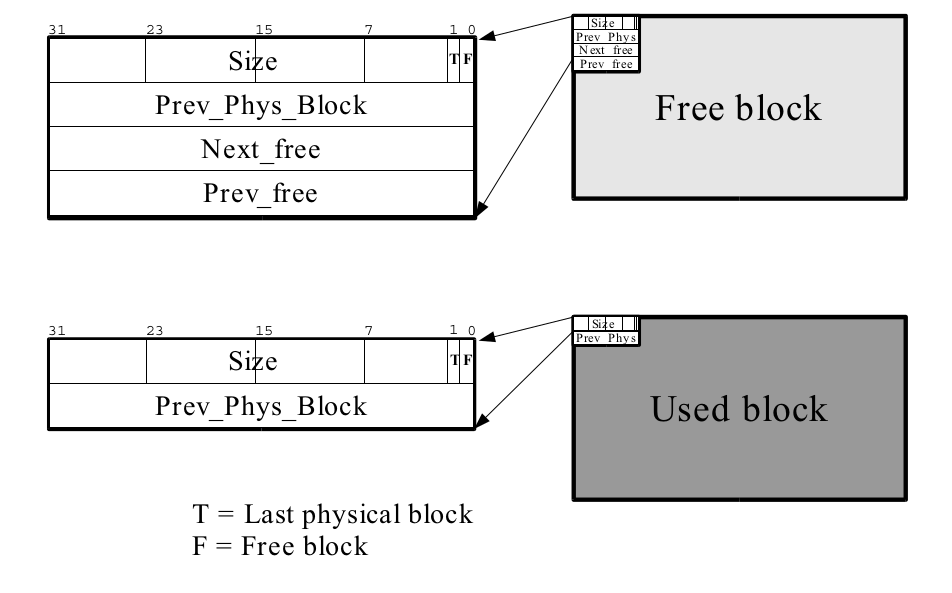
\includegraphics[width=0.65\textwidth]{figures/blockheader_reference.png}
    \caption{Representation of free and allocated block headers. (Taken from~\cite{TLSF}).}
    \label{fig:blockheader_reference}
\end{figure}

The work of the TLSF authors primarily focuses on explicit low-level allocation primitives, with no explicit consideration for garbage collection. Therefore, investigating how TLSF can be adapted to fit into the context of garbage collection represents a crucial and promising avenue for advancing its development.

%%% Local Variables:
%%% mode: latex
%%% TeX-master: "main"
%%% End:
